% manuscript-sha256: a4a7d840b11e912896032aebc9ead95f7978c0e6f60656f44645c6d8fadf593b
% Options for packages loaded elsewhere
\PassOptionsToPackage{unicode}{hyperref}
\PassOptionsToPackage{hyphens}{url}
\PassOptionsToPackage{dvipsnames,svgnames,x11names}{xcolor}
\documentclass[
  11pt,
]{article}
\usepackage{xcolor}
\usepackage[margin=25mm]{geometry}
\usepackage{amsmath,amssymb}
\setcounter{secnumdepth}{-\maxdimen} % remove section numbering
\usepackage{iftex}
\ifPDFTeX
  \usepackage[T1]{fontenc}
  \usepackage[utf8]{inputenc}
  \usepackage{textcomp} % provide euro and other symbols
\else % if luatex or xetex
  \usepackage{unicode-math} % this also loads fontspec
  \defaultfontfeatures{Scale=MatchLowercase}
  \defaultfontfeatures[\rmfamily]{Ligatures=TeX,Scale=1}
\fi
\usepackage{lmodern}
\ifPDFTeX\else
  % xetex/luatex font selection
  \setmainfont[]{Latin Modern Roman}
  \setmonofont[]{Latin Modern Mono}
\fi
% Use upquote if available, for straight quotes in verbatim environments
\IfFileExists{upquote.sty}{\usepackage{upquote}}{}
\IfFileExists{microtype.sty}{% use microtype if available
  \usepackage[]{microtype}
  \UseMicrotypeSet[protrusion]{basicmath} % disable protrusion for tt fonts
}{}
\makeatletter
\@ifundefined{KOMAClassName}{% if non-KOMA class
  \IfFileExists{parskip.sty}{%
    \usepackage{parskip}
  }{% else
    \setlength{\parindent}{0pt}
    \setlength{\parskip}{6pt plus 2pt minus 1pt}}
}{% if KOMA class
  \KOMAoptions{parskip=half}}
\makeatother
\usepackage{longtable,booktabs,array}
\usepackage{calc} % for calculating minipage widths
% Correct order of tables after \paragraph or \subparagraph
\usepackage{etoolbox}
\makeatletter
\patchcmd\longtable{\par}{\if@noskipsec\mbox{}\fi\par}{}{}
\makeatother
% Allow footnotes in longtable head/foot
\IfFileExists{footnotehyper.sty}{\usepackage{footnotehyper}}{\usepackage{footnote}}
\makesavenoteenv{longtable}
\usepackage{graphicx}
\makeatletter
\newsavebox\pandoc@box
\newcommand*\pandocbounded[1]{% scales image to fit in text height/width
  \sbox\pandoc@box{#1}%
  \Gscale@div\@tempa{\textheight}{\dimexpr\ht\pandoc@box+\dp\pandoc@box\relax}%
  \Gscale@div\@tempb{\linewidth}{\wd\pandoc@box}%
  \ifdim\@tempb\p@<\@tempa\p@\let\@tempa\@tempb\fi% select the smaller of both
  \ifdim\@tempa\p@<\p@\scalebox{\@tempa}{\usebox\pandoc@box}%
  \else\usebox{\pandoc@box}%
  \fi%
}
% Set default figure placement to htbp
\def\fps@figure{htbp}
\makeatother
\setlength{\emergencystretch}{3em} % prevent overfull lines
\providecommand{\tightlist}{%
  \setlength{\itemsep}{0pt}\setlength{\parskip}{0pt}}
\usepackage{bookmark}
\IfFileExists{xurl.sty}{\usepackage{xurl}}{} % add URL line breaks if available
\urlstyle{same}
\hypersetup{
  colorlinks=true,
  linkcolor={Maroon},
  filecolor={Maroon},
  citecolor={Blue},
  urlcolor={Blue},
  pdfcreator={LaTeX via pandoc}}

\author{}
\date{}

\usepackage{xurl}
\usepackage{newunicodechar}
\usepackage{needspace}
\usepackage{pdflscape}
\newunicodechar{∎}{\ensuremath{\square}}
\newunicodechar{→}{\ensuremath{\to}}
\newunicodechar{←}{\ensuremath{\leftarrow}}
\newunicodechar{↦}{\ensuremath{\mapsto}}
\newunicodechar{≠}{\ensuremath{\ne}}
\newunicodechar{⊆}{\ensuremath{\subseteq}}
\newunicodechar{∩}{\ensuremath{\cap}}
\newunicodechar{∪}{\ensuremath{\cup}}
\newunicodechar{∅}{\ensuremath{\varnothing}}
\newunicodechar{∈}{\ensuremath{\in}}
\newunicodechar{∉}{\ensuremath{\notin}}
\newunicodechar{⊔}{\ensuremath{\sqcup}}
\newunicodechar{−}{\ensuremath{-}}
\newunicodechar{ε}{\ensuremath{\varepsilon}}
\newunicodechar{α}{\ensuremath{\alpha}}
\newunicodechar{β}{\ensuremath{\beta}}
\newunicodechar{γ}{\ensuremath{\gamma}}
\newunicodechar{²}{\ensuremath{{}^2}}
\newunicodechar{³}{\ensuremath{{}^3}}
\newunicodechar{φ}{\ensuremath{\varphi}}
\newunicodechar{Σ}{\ensuremath{\Sigma}}
\newunicodechar{Γ}{\ensuremath{\Gamma}}
\setlength{\emergencystretch}{3em}
\begin{document}

\begin{center}
{\LARGE\bfseries From Pre-Genesis to MSS-N\par}
Jeremy H. Carroll\par
2026-10-09\par
Version 1.0.0\par
\end{center}

\subsection{Abstract}\label{abstract}

An uninterpreted inscription supplies no admission policy, observation
rule or mathematical realization on its own. This paper joins the
recorded Pre-Genesis trials to the S(n) presentation account and the
Minimal Symbol System atlas. It distinguishes supplied text, admitted
objects, reports, grammar profiles and proposed capability targets.
Exact report reconstruction, finite demand accounting, typed recovery
and alphabet extension provide separate preservation criteria. At the
chain-complex level, a retraction prevents an extension from killing an
old nonzero homology class. Graph and word examples show why recovering
syntax, distinguishing observations and repairing topology require
different proofs. The companions construct integral component and
triangle homology, canonical free-word reduction and an exact rational
Bell-mixture obstruction. The three recorded model runs are historical
examples with missing model metadata; they supply no success rates. The
consolidation retains corrected source claims and withdrawn physical
interpretations, and identifies the precise scope of its Lean, Python
and Rust companions. As an entry companion to the Witnessed Difference
Programme monograph, it prepares the report, recovery and repair
contracts used by that work's later conditional finite-QM constructions.

\subsection{\texorpdfstring{1. Starting before
\texttt{\textless{}\textgreater{}}}{1. Starting before \textless\textgreater{}}}\label{starting-before}

The first question is what has been supplied and what has been licensed
to happen with it. The author, reader and computer already use a
metalanguage. This paper makes that fact explicit; it does not describe
an observer-free creation from nothing.

\begin{longtable}[]{@{}
  >{\raggedright\arraybackslash}p{(\linewidth - 4\tabcolsep) * \real{0.3333}}
  >{\raggedright\arraybackslash}p{(\linewidth - 4\tabcolsep) * \real{0.3333}}
  >{\raggedright\arraybackslash}p{(\linewidth - 4\tabcolsep) * \real{0.3333}}@{}}
\toprule\noalign{}
\begin{minipage}[b]{\linewidth}\raggedright
Condition
\end{minipage} & \begin{minipage}[b]{\linewidth}\raggedright
Host-level description
\end{minipage} & \begin{minipage}[b]{\linewidth}\raggedright
What has not followed
\end{minipage} \\
\midrule\noalign{}
\endhead
\bottomrule\noalign{}
\endlastfoot
Absent input & No payload was supplied, for example \nolinkurl{None} in a
declared option type. & No object-level empty word or ground has been
produced. \\
Empty word & The word epsilon in a declared free monoid has length zero.
& It need not be accepted by a selected grammar start. \\
Literal \texttt{\textless{}\textgreater{}} & Two ASCII characters,
possibly one opaque token under a stated lexer. & Neither an empty set
nor a singleton carrier is forced. \\
Admitted ground & A named initial object under an explicit regime
definition. & Its carrier, operations and permitted transitions still
need definitions. \\
\end{longtable}

``Before'' here marks the order of questions in the account. It is not a
derivation of physical time. Even writing \nolinkurl{None} presupposes a
host capable of representing absence. Likewise, a grammar production
cannot demonstrate that there is no grammar in the metalanguage in which
that production was written.

Let a declared transition system have state set X and transition
relation T. If T is empty, no state has a T-successor. This follows from
the definition of an empty relation. It does not say that an external
caller cannot provide more data, or that every later rule is prohibited.
External supply and admission are events whose effects must be
specified.

\subsubsection{1.1 Reading toward the WDP
monograph}\label{reading-toward-the-wdp-monograph}

This paper supplies the entrance to \emph{The Witnessed Difference
Programme --- From Finite Distinction to Witnessed Measurement}.
Pre-Genesis asks what was supplied, admitted and retained. S(n)
separates presentation stages from mathematical degree. MSS-N supplies a
vocabulary of proposed targets whose realizations need explicit
contracts. The report and graph examples below make those contracts
concrete before the monograph introduces its richer repair and observer
models.

The contribution presented here is the organized passage from admission
and observation questions to typed mathematical preservation and repair,
with inspectable formal constructions and executable contracts. Standard
algebraic results are identified at their points of use. The route is
evaluated through its explicit maps, hypotheses and worked examples.

Read §§4--5 for sufficient reports, §§9--12 for typed recovery, and §13
for the preservation/repair distinction. Section 17.1 then gives the
chapter handoff. The \href{docs/monograph_route.md}{reading route and
edition binding} identify the companion draft. The later quantum
carriers and readout rules are constructed in that monograph under its
stated additional assumptions.

\subsection{2. What the Pre-Genesis trials actually
recorded}\label{what-the-pre-genesis-trials-actually-recorded}

The \href{docs/sources/pre_genesis/readme.txt}{Pre-Genesis strand}
contains the experiment design, Trial 1, Trial 2 and a full-history
replay. Its \href{docs/sources/pre_genesis/02_trial_record.txt}{trial
record} points to the original transcripts. The prompts withheld the
intended comparison theories and asked the model to distinguish external
presentation from internal expressibility. ``No move is forced'' was an
admissible outcome. The next inscription was not prescribed as a
successful rediscovery of an existing calculus.

The record supports the following limited observations:

\begin{longtable}[]{@{}
  >{\raggedright\arraybackslash}p{(\linewidth - 4\tabcolsep) * \real{0.3333}}
  >{\raggedright\arraybackslash}p{(\linewidth - 4\tabcolsep) * \real{0.3333}}
  >{\raggedright\arraybackslash}p{(\linewidth - 4\tabcolsep) * \real{0.3333}}@{}}
\toprule\noalign{}
\begin{minipage}[b]{\linewidth}\raggedright
Event
\end{minipage} & \begin{minipage}[b]{\linewidth}\raggedright
Recorded behavior
\end{minipage} & \begin{minipage}[b]{\linewidth}\raggedright
Evidential boundary
\end{minipage} \\
\midrule\noalign{}
\endhead
\bottomrule\noalign{}
\endlastfoot
Bare marks and punctuation controls & A fenced prompt elicited familiar
interpretations; raw controls elicited different replies. & The runs did
not isolate every causal difference between conditions. \\
No declared continuation rule & All three runs said that a successor was
not forced; some proposed a continuation under an added assumption. & A
proposal and its adoption are different events. \\
\texttt{\textless{}a\textgreater{}} supplied after
\texttt{\textless{}\textgreater{}} & Replies differed between
presentation-relative and inscription-relative readings of identity. &
The identity convention had not been fixed. \\
A separation task about \texttt{\textless{}a\textgreater{}} and
\texttt{\textless{}ab\textgreater{}} & A reply treated observational
indistinguishability as identification; another used a stale account of
the current state. & Lack of a distinguishing operation does not itself
install an object-language equality rule. \\
Truncated audit versus replay & An auditor examining only the local
response missed a historical-state mismatch. & Local consistency alone
did not establish consistency with the adopted history. \\
\end{longtable}

Trial 1 also bundled steps and fenced controls that the design had
intended to send separately and raw. These are recorded design
deviations. The model identifier, settings and dates were not recorded.
There were no host-checker verdicts on the replies and no live PFP
evaluation. The earlier invented ``50 trials'' table is not part of the
evidence used here. No rate, benchmark advantage or theory-rediscovery
claim follows from this record.

The
\href{docs/sources/pre_genesis/04_named_failure_modes.txt}{failure-mode
chapter} names semantic overcompletion, premature relation, false
provenance, lost state, stale certification and bundled extension. These
are retrospective descriptions. Naming a failure does not implement a
detector for it.

\subsection{3. Six operations that must remain
distinct}\label{six-operations-that-must-remain-distinct}

The trials become easier to interpret when the following operations have
separate signatures and records:

\begin{longtable}[]{@{}
  >{\raggedright\arraybackslash}p{(\linewidth - 2\tabcolsep) * \real{0.5000}}
  >{\raggedright\arraybackslash}p{(\linewidth - 2\tabcolsep) * \real{0.5000}}@{}}
\toprule\noalign{}
\begin{minipage}[b]{\linewidth}\raggedright
Operation
\end{minipage} & \begin{minipage}[b]{\linewidth}\raggedright
Meaning in a declared host
\end{minipage} \\
\midrule\noalign{}
\endhead
\bottomrule\noalign{}
\endlastfoot
Mention & Refer to an inscription or possible object in a discussion. \\
Supply & Deliver a payload to an interface. \\
Designate & Identify which presentation is currently under
consideration. \\
Admit & Add a datum, form, instance or rule according to an admission
policy. \\
Retain & Preserve an admitted object or event for subsequent use. \\
Operate & Apply an admitted transformation with stated preconditions. \\
\end{longtable}

A response proposing \texttt{\textless{}a\textgreater{}} does not
establish that \texttt{\textless{}a\textgreater{}} was adopted. A later
task that mentions \texttt{\textless{}ab\textgreater{}} need not erase
\texttt{\textless{}a\textgreater{}}. A checker cannot reconstruct these
facts from punctuation alone; it needs event semantics and enough of the
event record.

The trial method is consequently modest: keep discovery prompts free of
expected solutions, preserve the exact controls, separate steps, record
adoption explicitly, and bind an audit to its actual context. These are
design lessons from the record, not experimentally established universal
remedies.

\subsection{4. Observation-relative
difference}\label{observation-relative-difference}

Let A be a declared carrier and O a family of functions on A. Write

\[
x\sim_O y \quad\Longleftrightarrow\quad
   o(x)=o(y)\text{ for every }o\in O.
\]

Equality here is metatheoretic equality in each observation's codomain.
If O is empty, every pair is equivalent. This does not imply that the
inscription strings are equal or that the regime contains an equality
operator.

\textbf{Proposition 1 --- separation cannot be recovered from a
collapsed quotient.} Suppose x and y have the same O-profile, while a
task f requires f(x) different from f(y). No function on the current
observational quotient can answer f on all inputs.

\textbf{Proof.} The quotient map q sends x and y to the same class. If
f=g composed with q, then f(x)=g(q(x))=g(q(y))=f(y), a contradiction.
Therefore a representation supporting this task must preserve more
information than q preserves. This may be achieved by adding an
observation that separates the pair. The proposition does not select
that observation. ∎

For \texttt{\textless{}a\textgreater{}} and
\texttt{\textless{}ab\textgreater{}}, a predicate for presence of
\nolinkurl{b} and a predicate for payload length greater than one both
separate the pair, under a supplied string decoder. They disagree on
\texttt{\textless{}aa\textgreater{}}. Full inscription identity also
separates the pair and retains additional information. These are
alternative admitted solutions, not capabilities obtained without a
decoder or comparison operation.

\subsection{5. A history projection can destroy the
answer}\label{a-history-projection-can-destroy-the-answer}

Let \(H\) be a set of admissible histories, \(\sigma:H\to S\) the state
or protected answer required by a task, and \(\pi:H\to V\) the report
shown to an auditor.

\textbf{Theorem 2 --- history report criterion.} An answer map
\(A:\pi(H)\to S\) satisfying \(A(\pi(h))=\sigma(h)\) for every
\(h\in H\) exists if and only if

\[
\pi(h)=\pi(h')\quad\Longrightarrow\quad\sigma(h)=\sigma(h').
\]

When it exists, it is unique on the report image. In particular, two
histories with the same report and different required answers rule out
an auditor that answers correctly on all admissible histories while
seeing only that report.

\textbf{Proof.} A factorization gives
\(\sigma(h)=A(\pi(h))=A(\pi(h'))=\sigma(h')\). Conversely, define
\(A(\pi(h))=\sigma(h)\); the displayed condition makes this
well-defined. Every member of \(\pi(H)\) has this form, so the factor is
unique. For a finite listed history population with decidable report
equality, the construction is executable: find the first matching report
and return that history's answer. Extending the map outside \(\pi(H)\)
requires a chosen answer there; no such extension is needed for
reconstruction on admissible inputs. ∎

The carrier-general criterion and uniqueness on the report image are
mechanized as \nolinkurl{PreMssn.history_report_criterion} and
\nolinkurl{history_factor_unique} in \href{lean4/Paper.lean}{the Lean
companion}. The existence direction uses \nolinkurl{Classical.choice}; the
finite listed-history reconstruction in the Python and Rust companions
is constructive.

This is an information-loss theorem, not a theorem that every task
requires every raw token of history. A sufficient state summary may
preserve \(\sigma\). Conversely, more context alone does not guarantee
that an auditor will use it correctly. Raw history retention is a useful
provenance policy; task-sufficient reconstruction is the mathematical
requirement.

The local response in the trials could be consistent with its asserted
premise and still be inappropriate for the adopted state. Checking
internal steps and checking the binding of their premises to the actual
history are separate tasks. The report criterion makes this distinction
precise for any specified answer function on admissible histories.

\subsection{6. The indices and layers}\label{the-indices-and-layers}

\begin{longtable}[]{@{}
  >{\raggedright\arraybackslash}p{(\linewidth - 4\tabcolsep) * \real{0.3333}}
  >{\raggedright\arraybackslash}p{(\linewidth - 4\tabcolsep) * \real{0.3333}}
  >{\raggedright\arraybackslash}p{(\linewidth - 4\tabcolsep) * \real{0.3333}}@{}}
\toprule\noalign{}
\begin{minipage}[b]{\linewidth}\raggedright
Symbol or object
\end{minipage} & \begin{minipage}[b]{\linewidth}\raggedright
Meaning
\end{minipage} & \begin{minipage}[b]{\linewidth}\raggedright
Separate quantity
\end{minipage} \\
\midrule\noalign{}
\endhead
\bottomrule\noalign{}
\endlastfoot
S(n) & A presentation stage in the specified admission account. & The
number of glyphs or a homotopy degree. \\
k & Alphabet size under a declared token policy. & Number of decoded
objects or operations. \\
p & Grammar/profile and public start. & Semantic interpretation or
evaluation verdict. \\
MSS-m & An externally specified atlas target. & A native Genesis stage
or a completed lift. \\
\(H_j\) & Homology in degree j of a declared complex. & Stage n or
active-demand count. \\
C(m), D & A declared coverage measure and length of a contiguous
licensed chain. & One another; neither is inferred from the number of
folders. \\
\end{longtable}

For example, S(2) in the teaching crosswalk records retained but
observationally collapsed data. MSS-2 is a target about relations.
Equating them by their numerals silently changes the object under
discussion.

Four responsibilities remain distinct: native admissions; mathematical
representations; downstream interpretations; and verification/evidence
machinery. A Lean proof, a Python calculation and a SQL view may refer
to related structures, but shared terminology does not prove that they
evaluate the same property.

\Needspace{430pt}
\subsection{7. The finite-stage
crosswalk}\label{the-finite-stage-crosswalk}

The \href{docs/sources/genesis_education.txt}{Genesis account} is the
source for admission, observation, candidate costs and the
sealed/post-seal distinctions. The following is a presentation
crosswalk, not a claim that the displayed glyphs derive their own
semantics or that every row is forced independently of policy.

\begin{longtable}[]{@{}
  >{\raggedright\arraybackslash}p{(\linewidth - 4\tabcolsep) * \real{0.3333}}
  >{\raggedright\arraybackslash}p{(\linewidth - 4\tabcolsep) * \real{0.3333}}
  >{\raggedright\arraybackslash}p{(\linewidth - 4\tabcolsep) * \real{0.3333}}@{}}
\toprule\noalign{}
\begin{minipage}[b]{\linewidth}\raggedright
Stage
\end{minipage} & \begin{minipage}[b]{\linewidth}\raggedright
Presentation question
\end{minipage} & \begin{minipage}[b]{\linewidth}\raggedright
Required qualification
\end{minipage} \\
\midrule\noalign{}
\endhead
\bottomrule\noalign{}
\endlastfoot
S(0) & What is received as the opaque ground inscription? &
\texttt{\textless{}\textgreater{}} has no inherited object-language
meaning. Ground inertia is relative to the specified rules. \\
S(1) & Has a newly supplied mark been consumed or admitted? & Supply
alone may be an internal no-op. \\
S(2) & What data have been retained, and which profiles remain equal? &
Host-level multiplicity does not create an internal distinguishing
context. \\
S(3) & How can a supplied pair-separation task be met? & The cost-two
result uses a particular response grammar and cost; it is not a
universal witness count. \\
S(4) & Have the relevant pairs been separated under the chosen closure
policy? & Pair closure needs its finite-carrier and preservation
assumptions. \\
S(5) & Where does the next requirement or fresh datum come from? &
External continuation is a declared policy, not an endogenous generator
proved by saturation. \\
S(6) & How are old presentations represented and recovered after an
extension? & Typed maps and their preservation laws must be supplied and
checked. \\
\end{longtable}

A branching set of tied responses is not automatically a linear tower. A
chosen cost order, equivalence and continuation policy select or retain
its branches. Subsequent atlas targets may ask for graphs, algebra,
categories or geometry. Their presence in the atlas does not establish
that the native process has reached them.

\subsubsection{7.1 Where the HoTT interpretation
entered}\label{where-the-hott-interpretation-entered}

The Pre-Genesis trials did not derive homotopy type theory (HoTT) from
the inscriptions. The S(n) account considered a connection with
Postnikov towers, conditional on supplying a topological realization and
its preservation maps. The MSS-N account explicitly introduced Genesis,
HoTT and category theory as three mathematical lenses. Its
types-as-spaces and identity-path vocabulary was an additional
interpretation, not a conclusion of the trial record. The
\href{docs/references.md}{source reader} identifies these historical
passages.

The current Lean constructions concern ordinary equality, algebraic
chain complexes and quotient groups. A chain homotopy is a relation
between chain maps; it does not by itself construct a HoTT identity type
or a univalent universe. The corrected account therefore retains the
mathematical connections while requiring a separate construction for any
claimed derivation of HoTT.

\subsection{8. Active demands, receipt sets and ordered
histories}\label{active-demands-receipt-sets-and-ordered-histories}

Let \(W_n\) be a finite register of active demands. A demand identifies
its carrier, protected condition, witness data and activity predicate.
It is not simply a label such as ``curvature'' or ``missing structure.''
Let \(D_{n+1}\) be the demands discharged in a step and \(B_{n+1}\) the
demands introduced. Assume

\[
D_{n+1}\subseteq W_n,\qquad
B_{n+1}\cap(W_n\setminus D_{n+1})=\varnothing,
\]

and define

\[
W_{n+1}=(W_n\setminus D_{n+1})\sqcup B_{n+1}.
\]

\textbf{Proposition 3 --- finite demand accounting.} With \(s_n=|W_n|\),
\(d_{n+1}=|D_{n+1}|\) and \(b_{n+1}=|B_{n+1}|\),

\[
s_{n+1}=s_n-d_{n+1}+b_{n+1}.
\]

\textbf{Proof.} Subset removal gives
\(|W_n\setminus D_{n+1}|=|W_n|-|D_{n+1}|\). Disjoint union then adds
\(|B_{n+1}|\). ∎

This identity does not prove which demands an engine actually carries.
In particular, the previously displayed sequence (0,1,1,1,0,1,1) follows
from one chosen assignment of singleton demands to the crosswalk. It is
an illustrative ledger, not a universal native survivor sequence or a
physical observable.

A cumulative receipt set \(H_{n+1}=H_n\cup C_{n+1}\) has nondecreasing
cardinality. An ordered event log additionally retains order and
multiplicity. Neither is \(W_n\). An empty active register need not
erase receipts, imply thermodynamic equilibrium, or prove that every
possible future question has been answered. Adding two map symbols does
not imply two active demands or two newly admitted carrier elements.

\subsection{9. Binary support and observation
refinement}\label{binary-support-and-observation-refinement}

An inhabited irreflexive relation R(a,b) forces a≠b, by the
irreflexivity argument below. Indeed, equality a=b would turn the
witness into R(a,a), contradicting irreflexivity. This gives two
endpoints for that edge, not two observers or two certificate
occurrences. The pointed graph D2 with vertices 0 and 1 and the single
edge 0→1 has exactly one endpoint-preserving map to a specified pair
(a,b); that map preserves the edge. This elementary pointed property
does not make D2 initial in an unspecified category of all possible
systems.

Suppose q:A→O identifies a and b. If a supplied tag t:A→\{0,1\} has
t(a)=0 and t(b)=1, define q'(x)=(q(x),t(x)). Then q'(a)≠q'(b), while
projection to the first component recovers q. Both claims follow
directly from equality of ordered pairs. The tag and its construction
are supplied data. A method for finding tags is a separate algorithmic
obligation.

For several required pairs, form a conflict graph on A. A tag assignment
separating every edge is a proper coloring. Thus the number of tag
values needed for many pairwise constraints need not remain two: a
three-clique needs three colors. The constraints remain binary without
implying a globally binary solution space.

\subsection{10. Typed recovery on the old
image}\label{typed-recovery-on-the-old-image}

Let u:A→B be a proposed lift and let

\[
\widehat r:B\to A+\{\mathrm{NON\_DESCENT}\}
\]

be a typed recovery map. The old-image law is

\[
\widehat r(u(a))=\mathrm{inl}(a)\quad(a\in A).
\]

\textbf{Proposition 4 --- injectivity.} This law implies that u is
injective. If u(a)=u(a'), applying the recovery map gives
inl(a)=inl(a'), hence a=a'. ∎

The law alone says nothing about off-image inputs. A checker intended to
reject all of them needs the additional specification

\[
b\notin\operatorname{im}(u)\;\Longrightarrow\;
\widehat r(b)=\mathrm{inr}(\mathrm{NON\_DESCENT}).
\]

It also needs a way to decide the image condition within its declared
domain and budget. That is immediate for some finite presentations and
not a general computability theorem.

Two further qualifications prevent stronger promises from being
inferred:

\begin{itemize}
\tightlist
\item
  \textbf{Observation preservation needs a commuting condition.} For old
  observation q:A→O and new observation q':B→O, require q' composed with
  u=q, or provide a declared transport to the old report space.
  Recovering a term does not by itself prove that a new evaluator uses
  the old observations.
\item
  \textbf{Repair needs its own proof.} An identity embedding has a
  perfect old-image law and can leave every original obstruction
  unchanged.
\end{itemize}

The pair is not generally an involution. Moreover, u composed with r-hat
is not even a map B→B until handling of the refusal summand has been
defined. No global preservation of all certificates follows from a
successful term round trip alone.

The current \href{lean4/SnCarrier.lean}{SnCarrier model} restricts the
section to \nolinkurl{BasePresentation}: ground, supplied mark, retained
pair, directed cut and simplex cut. Nested lifts, retractions and
refusal tokens are outside this source type. The theorem
\nolinkurl{SnTheorems.old_image_base} establishes the recovery equation
for every base constructor and every stage. \texttt{Carrier\ n} is
\texttt{Fin\ (carrierCard\ n)}, and \nolinkurl{ground_carrier_empty}
establishes that the index-zero carrier is empty. These definitions
correct the older unrestricted fallback and cardinality-table mismatch
described by the predecessor draft. They establish the declared local
model, rather than a correspondence theorem for every parser or source
regime.

\subsection{11. Formal languages and conditional expressive
capacity}\label{formal-languages-and-conditional-expressive-capacity}

A symbol system must declare terminal spellings, tokenization, grammar,
public start, layout policy, identity policy, annotation decoding and
allowed manipulations. These eight choices determine what an inscription
does.

For the familiar alphabet \(\Gamma_{38}\), the glyph inventory comprises
26 lowercase Latin letters, ten decimal digits and \texttt{\textless{}},
\texttt{\textgreater{}}. Some MSS grammar profiles add punctuation or
Unicode; they are not confined to these 38 characters.

Keep three relations separate:

\[
E\subseteq V\times V,\qquad
\to_{\rm rewrite}\;\subseteq\Sigma^*\times\Sigma^*,\qquad
q:V\to O.
\]

They represent an encoded relation, rewrites between inscriptions and an
observation map respectively. A change in any one need not change the
others.

With repetition admitted, the one-letter language \(a^+\) supports
positive unary counting under the length decoder. Including epsilon
gives \(a^*\) and a representation of zero. With two letters,
concatenation is noncommutative: ab and ba are different words. A
declared binary decoder can use any two distinct printed letters. A
relation may be encoded by positions or a table without an arrow glyph.
These are conditional constructions, not semantic resources supplied by
alphabet size alone.

\subsubsection{11.1 Free monoids and numeral
decoders}\label{free-monoids-and-numeral-decoders}

\textbf{Theorem 5.} Free monoids on finite alphabets of different sizes
are not isomorphic.

\textbf{Proof.} In a free monoid, the nonidentity elements that cannot
be factored as a product of two nonidentity elements are exactly the
one-letter words. A monoid isomorphism preserves identity and this
indecomposability property in both directions. It therefore induces a
bijection of the generating alphabets. Their sizes must agree. ∎

Thus binary and decimal string monoids are not isomorphic. Decoders can
map their strings onto the same natural numbers without making the
string monoids identical. A fixed-width binary encoding of decimal
digits is injective under concatenation, but not onto the binary free
monoid.

Likewise, discrete categories with two and 26 objects are not
equivalent: all isomorphism classes are singletons, and an equivalence
would have to match those classes bijectively.

\subsubsection{11.2 Three recovery constructions with different
types}\label{three-recovery-constructions-with-different-types}

For alphabets A contained in B, language inclusion and restriction are

\[
\ell:\mathcal P(A^*)\to\mathcal P(B^*),\quad\ell(L)=L,
\qquad r(M)=M\cap A^*.
\]

Then \(r(\ell(L))=L\). This is a retraction of sets of words.

For individual words, exact recovery of old words can instead return the
same word if it is in A\emph{, and a typed refusal otherwise. A total
erasure homomorphism h:B}→A* is another choice: map each new letter to
epsilon and concatenate. It recovers every old word but loses new
letters and their positions. These are three distinct contracts, not one
overloaded ``down-map.''

No abelian category of ordinary formal languages has been specified
here. An Ext calculation cannot be inferred from language restriction.
Even in an abelian category, a split extension is one zero extension
class; it does not show that an entire Ext group vanishes.

\subsection{12. Manipulations and actual information
loss}\label{manipulations-and-actual-information-loss}

A renaming f:A→B has a two-sided inverse on the entire codomain B
exactly when it is bijective. Recovery of source letters from the image
f(A) only requires injectivity. Mapping both c and d to d collapses ac
and ad. This is independent of whether the resulting word is
grammatically well formed.

For the code a↦0 and b↦00, the different source words aa and b both
encode as 00; ab and ba both encode as 000. A decoder cannot recover the
source universally without additional retained information or a
restricted source domain.

For declared directed-edge syntax:

\begin{longtable}[]{@{}ll@{}}
\toprule\noalign{}
Inscription & Represented edge \\
\midrule\noalign{}
\endhead
\bottomrule\noalign{}
\endlastfoot
\texttt{a\textgreater{}b} & a→b \\
\texttt{b\textgreater{}a} & b→a \\
\texttt{a\textless{}b} & b→a \\
\texttt{b\textless{}a} & a→b \\
\end{longtable}

Reversing the vertex sequence and every arrow in
\texttt{a\textgreater{}b\textgreater{}c} gives
\texttt{c\textless{}b\textless{}a} and preserves its directed edge
multiset. It changes the traversal order. A checker must name whether it
protects the edge multiset, the ordered trace, annotations, or exact
source bytes. AST recovery and byte recovery are different questions.

\subsection{13. Finite graphs and the homological
obstruction}\label{finite-graphs-and-the-homological-obstruction}

For a finite directed graph, regard the underlying graph as a
one-dimensional cell complex and define

\[
C_1=\mathbb Z^E\xrightarrow{\partial_1}C_0=\mathbb Z^V,
\qquad\partial_1(e)=t(e)-s(e).
\]

If V is nonempty and the underlying undirected graph has c components,
then \(H_0\cong\mathbb Z^c\) and \(\widetilde H_0\cong\mathbb Z^{c-1}\).
The maximal component count \textbar V\textbar{} occurs when no edge
joins distinct vertices; self-loops do not affect it. Adding an edge
reduces the component count only when it joins previously distinct
components. It does not separate a and b under an unchanged observation
q with q(a)=q(b).

These standard graph and homology facts use the conventions in
\href{https://pi.math.cornell.edu/~hatcher/AT/AT.pdf}{Hatcher's
\emph{Algebraic Topology}}, §1.A, Proposition 2.7 and §2.A.

Formal negative coefficients do not authorize reverse physical
traversal. In a CW graph, a self-loop has zero boundary and can generate
nonzero \(H_1\). It is not a degenerate simplex solely because its
endpoints coincide; the model matters.

\subsubsection{13.1 The chain-retraction
obstruction}\label{the-chain-retraction-obstruction}

\textbf{Theorem 6.} Let \(i:C\to D\) and \(r:D\to C\) be chain maps with
\(r\circ i=\mathrm{id}_C\). Then \(H_j(i)\) is injective for every j. In
particular, i cannot kill a nonzero homology class of C.

\textbf{Proof.} If z is a cycle in C and i(z)=partial\_D b, then

\[
z=r(i(z))=r(\partial_D b)=\partial_C r(b).
\]

So z was already a boundary in C. Therefore the kernel of \(H_j(i)\) is
zero. ∎

This is the central preservation limit inherited from the MSS-N
monograph. It does not prohibit every useful extension; it identifies
incompatible promises. An extension may repair a cycle while preserving
inscriptions, labels or selected questions, but it cannot simultaneously
claim this chain-map retraction fixing all of C.

The obstruction persists when the retraction equation holds only up to
chain homotopy. The \href{lean4/ChainHomotopy.lean}{homotopy companion}
establishes that homotopic chain maps induce the same map on the
constructed homology quotient. A homotopy left inverse therefore still
induces a left inverse and forces injectivity. In particular, the filled
triangle below has no such homotopy retraction onto its unfilled
complex.

\subsubsection{13.2 Two isolated points}\label{two-isolated-points}

Let \(C_0=\mathbb Za\oplus\mathbb Zb\) and \(C_1=0\). Add an edge e with
\(\partial_D e=b-a\), obtaining D. A retraction fixing the original
vertices would have \(r_0=\mathrm{id}\) and \(r_1(e)=0\). The chain-map
equation would require \(b-a=\partial_C(0)=0\), contradicting the linear
independence of a and b in the free abelian group. The new edge kills
the old reduced zero-dimensional class, so the theorem applies.

\subsubsection{13.3 A triangle and an explicitly attached
face}\label{a-triangle-and-an-explicitly-attached-face}

Under label identity,
\texttt{a\textgreater{}b\textgreater{}c\textgreater{}a} represents edges
\(e_{ab},e_{bc},e_{ca}\). Their sum z has boundary
\((b-a)+(c-b)+(a-c)=0\). With no two-cells, \(H_1\) is generated by
\([z]\). Adjoining a face f with \(\partial_2 f=z\) makes z a boundary
and satisfies \(\partial_1\partial_2=0\). The inscription gave the
one-skeleton; the face is an additional declared object.

Killing this class prevents a chain-map retraction fixing the original
complex. It does not prove that an unrelated observational collision has
been resolved. Nor does one vanishing class show that every homology
group vanishes.

Chains and cochains must remain typed separately:
\(C^j=\operatorname{Hom}(C_j,\mathbb Z)\) and
\((d^j\varphi)(c)=\varphi(\partial_{j+1}c)\). Filling a chain is not the
same equation as finding a cochain primitive. Homological vanishing also
differs from null-homotopy: the commutator loop in the wedge of two
circles has zero abelianized homology class but is nontrivial in its
free fundamental group.

\begin{figure}
\centering
\pandocbounded{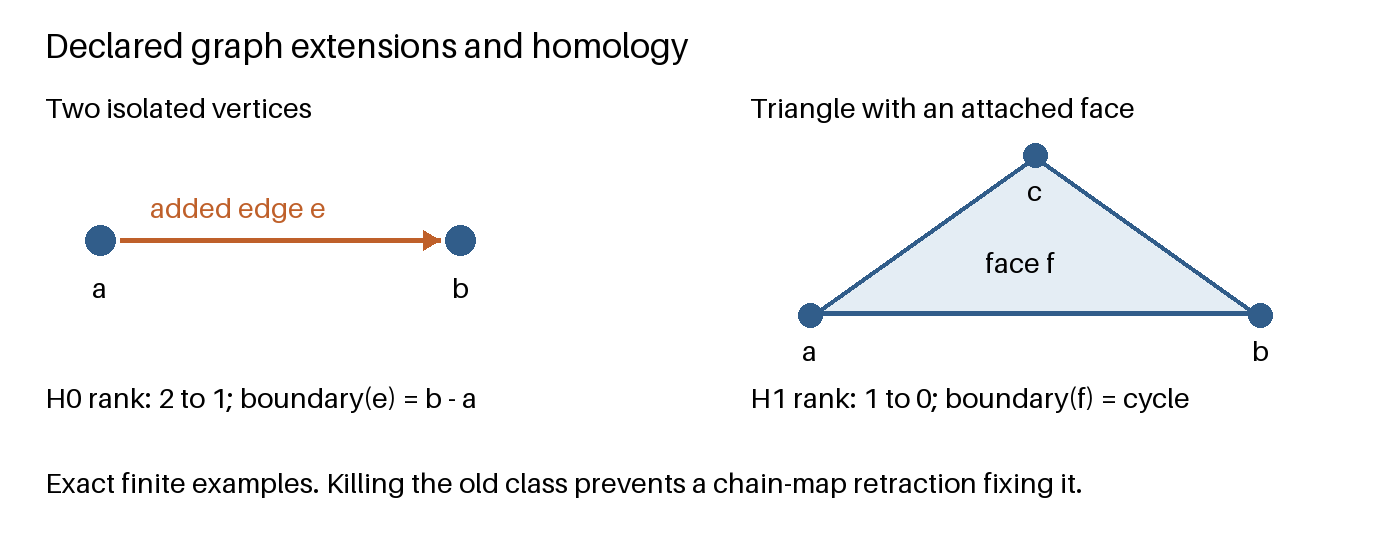
\includegraphics[keepaspectratio,alt={Two explicitly declared graph extensions. Killing the old class prevents a chain-map retraction fixing the old complex.}]{public_export/graph_extensions.png}}
\caption{Two explicitly declared graph extensions. Killing the old class
prevents a chain-map retraction fixing the old complex.}
\end{figure}

\subsubsection{13.4 Constructed homology groups and integral
classes}\label{constructed-homology-groups-and-integral-classes}

The \href{lean4/Homology.lean}{homology companion} constructs the cycle
subgroup, the equivalence relation modulo boundaries and its quotient
abelian group. It constructs the homomorphism induced by a chain map and
establishes the induced retraction equation. The theorem
\nolinkurl{induced_homology_injective} realizes Theorem 6 on these
quotient groups. Group laws, well-definedness and injectivity are proved
from the supplied additive-group and chain-map laws; they are not
assumed properties of a named homology object.

An integral test complex has three consecutive chain groups equal to
\(\mathbb Z\), with \(\partial_2(k)=mk\) and \(\partial_1=0\). Its
middle classes satisfy \([n]=[p]\) exactly when \(n=p+mk\) for some
integer k. The companion establishes that Euclidean remainders classify
these classes for every integer m, including m=0. At m=2, the class of 1
is nonzero and its double is zero. This is a constructed torsion
example, without assigning it to an undeclared surface. The shared
runtime encoding retains n when m=0 and otherwise returns the
nonnegative remainder modulo \(|m|\).

\subsubsection{13.5 The component group is
constructed}\label{the-component-group-is-constructed}

The \href{lean4/GraphHomology.lean}{graph companion} constructs integral
zero-chains as the free abelian group on vertices and one-chains as the
free abelian group on edges. Its boundary sends an edge to its target
minus its source. Connected components are the quotient of vertices by
the equivalence relation generated by edges, allowing reversal and
concatenation of paths.

The maps in \nolinkurl{h0ComponentIso} give mutually inverse homomorphisms
between the boundary quotient and the free abelian group on these
components. The construction also identifies that boundary quotient with
the kernel/image homology group of the graph's degree-zero chain
fragment. Thus the unreduced component statement in §13 has a
carrier-general companion, including empty graphs, loops and parallel
edges. The free abelian group's extension and uniqueness properties are
established from its term quotient; freeness is not a supplied
hypothesis.

The theorem \nolinkurl{vertex_class_eq_iff_connected} states that two
vertex generators give the same zero-dimensional class exactly when they
are connected. A loop's boundary is zero. In the finite replay, a
component is named by its least vertex and a zero-chain is sent to its
integer coefficient sum in each component. These coordinates preserve
component information and vanish on boundaries; they do not alter the
observation map q.

\subsubsection{13.6 Finite coordinates and constructive edge
retractions}\label{finite-coordinates-and-constructive-edge-retractions}

The \href{lean4/FiniteCoordinates.lean}{finite-coordinate construction}
identifies the free abelian group on a carrier enumerated by
\texttt{Fin\ c} with integer c-tuples. It transports this isomorphism to
the actual graph component group. For c=n+1, the augmentation kernel is
isomorphic to integer n-tuples: retain the last n coordinates and
recover the first as minus their sum. This establishes the displayed
reduced-rank formula from explicit inverse homomorphisms.

The \href{lean4/GraphExtensions.lean}{edge-extension construction}
establishes that adding an edge reduces the finite component count
exactly when its endpoints were previously disconnected. It also
establishes the maximal-count criterion and that a loop gives a nonzero
class in the graph complex with no two-cells.

More precisely, an added edge has a chain retraction fixing every old
zero-chain if and only if its endpoints were already connected. In the
connected case, \href{lean4/GraphRetraction.lean}{the construction}
sends the new edge to an integral old path chain with the same boundary
and fixes the old edges. In the disconnected case, its induced homology
map identifies two old distinct vertex classes, contradicting Theorem 6.

The \href{lean4/UnionComponents.lean}{component algorithm} merges label
fibers along the supplied edge list. Its labels agree exactly on
connected vertices and, equivalently, on equal vertex classes in H0.
Choosing the first matching vertex in a complete enumeration gives
actual component representatives and a basis for H0. With vertices
enumerated in increasing order, the construction establishes that the
selected representative is the least vertex in its component.

\subsubsection{13.7 Triangle classification and the nonabelian
distinction}\label{triangle-classification-and-the-nonabelian-distinction}

The \href{lean4/TriangleHomology.lean}{triangle construction}
establishes that every integral cycle has a unique form (k,k,k). Its
actual unfilled H1 quotient is isomorphic to the integers. Every cycle
becomes a boundary after the displayed face is attached, and the filled
H1 quotient is trivial. The attachment kills the old generator and has
no chain retraction fixing the old middle group. Noncycles are refused
by the runtime class encoder.

More generally, prescribe the face boundary as m times the triangle
cycle for any integer m. The \href{lean4/TriangleDegree.lean}{degree
construction} gives actual inverse homology maps to the integral
quotient complex, so its H1 classes are classified by integers modulo m.
At m=0 the full integer coordinate remains; at m=1 the group is trivial;
at m=2 the cycle has a nonzero order-two class. This is an algebraic
chain-complex construction, without an inferred surface realization.

The \href{lean4/Cochain.lean}{dual construction} forms cochains as
additive homomorphisms and coboundaries by precomposition. The chain
square-zero law implies the cochain square-zero law. An edge cochain
with coefficients (p,q,r) evaluates on the attached triangle face as
p+q+r. Pullback along a chain map reverses its direction. A chain
retraction gives a split surjection on cohomology in the inclusion
direction, as the dual construction establishes for arbitrary abelian
coefficient groups.

The \href{lean4/FreeGroup.lean}{free-group construction} is a term
quotient by the group laws with a proved unique homomorphism extension
property. Its commutator on two generators is nontrivial, as a finite
permutation interpretation detects. Abelianization has the unique
factorization property for maps into abelian groups. The
\href{lean4/FreeWord.lean}{reduction theorem} strengthens this witness:
two signed words represent the same group element exactly when adjacent
inverse cancellation gives the same reduced word. The reduction
algorithm terminates structurally and is idempotent.

The \href{lean4/WedgeHomology.lean}{two-loop chain complex} has H1
isomorphic to integer pairs. The commutator is nontrivial in the
constructed free group and has zero class in this actual homology group.
These algebraic and cellular constructions do not yet identify that free
group with the quotient of continuous based loops by homotopy in a
topological two-circle wedge. That comparison remains the cited
background statement and an open formal obligation.

\Needspace{260pt}
\subsection{14. Profiles, parsers and evidence
scope}\label{profiles-parsers-and-evidence-scope}

The \href{code/grammar/mssn.ebnf}{MSS grammar} defines the 22 explicit
starts inventoried in Appendix A. It supplies formation rules, not
physical models or admitted semantic operations.

\begin{longtable}[]{@{}
  >{\raggedright\arraybackslash}p{(\linewidth - 6\tabcolsep) * \real{0.2500}}
  >{\raggedright\arraybackslash}p{(\linewidth - 6\tabcolsep) * \real{0.2500}}
  >{\raggedright\arraybackslash}p{(\linewidth - 6\tabcolsep) * \real{0.2500}}
  >{\raggedright\arraybackslash}p{(\linewidth - 6\tabcolsep) * \real{0.2500}}@{}}
\toprule\noalign{}
\begin{minipage}[b]{\linewidth}\raggedright
Selected profile
\end{minipage} & \begin{minipage}[b]{\linewidth}\raggedright
\texttt{a\textgreater{}b\textgreater{}c\textgreater{}a}
\end{minipage} & \begin{minipage}[b]{\linewidth}\raggedright
\texttt{a0\textgreater{}b2\textgreater{}c1\textgreater{}a0}
\end{minipage} & \begin{minipage}[b]{\linewidth}\raggedright
Interpretation if a decoder is supplied
\end{minipage} \\*
\midrule\noalign{}
\endhead
\bottomrule\noalign{}
\endlastfoot
\nolinkurl{raw_glyphs} & Accepted & Accepted & Character sequence only. \\*
\nolinkurl{label_path} & Accepted & Accepted & Whole labels such as
\nolinkurl{a0} are identifiers. \\*
\nolinkurl{suffix_path} & Rejected & Accepted & A letter plus a required
digit suffix. \\*
\nolinkurl{glyph_path} & Accepted & Rejected & Single glyphs separated by
direction marks. \\*
\end{longtable}

An outer enclosure is not a universal requirement. Profile choice is
part of the input contract; a parser must not guess a favorable
interpretation after seeing an otherwise invalid candidate. Byte
sequences, Unicode scalar values, grapheme clusters and grammar tokens
also need separate counting conventions.

The historical inventory describes 22 starts alongside six retained
runtime profiles. That inventory is not evidence of 28 semantic
evaluators or a single shared resource limit. Recognition, AST
construction, decoding, evaluation and exact serialization are distinct
checks. A scalar syntax that accepts \texttt{a:1/0} still needs a
decoder to reject zero denominators unless the grammar itself has been
changed to exclude them.

The historical source manuscripts preserve the original parser
descriptions and historical codec example. They must be bound to their
profile and implementation revision before being used as current
protocol requirements.

\subsection{15. What a justified lift must
demonstrate}\label{what-a-justified-lift-must-demonstrate}

For a claim that an extension is necessary or minimal:

\begin{enumerate}
\def\labelenumi{\arabic{enumi}.}
\tightlist
\item
  State the failed predicate and protected observations or laws.
\item
  Specify admissible repairs within the current carrier and operations.
\item
  Establish that those repairs cannot meet the predicate, or report
  incomplete search if the budget prevents that conclusion.
\item
  Specify the extension class, equivalence and cost order.
\item
  Retain all tied minima unless an explicit selection policy is applied.
\item
  Check that each accepted extension meets the predicate and preserves
  the particular contract being claimed.
\end{enumerate}

A finite candidate census is exhaustive only for its declared domain. A
budget stop is not proof of obstruction. A declared successor, a
proposed lift and a licensed transition therefore have separate evidence
states. Exact names of runtime terminal values belong to the engineering
protocol's schema; combining papers does not create a new enum or claim
every runner already conforms.

Similarly, proposer, evaluator and authorizer are roles with different
inputs and responsibilities. Three agents are neither necessary nor
sufficient. A theorem that an already halted state is unchanged by
replay establishes that equation; it does not prove the authorization of
an active transition.

\subsection{16. Boundaries retained from the corrected
walkthrough}\label{boundaries-retained-from-the-corrected-walkthrough}

The following withdrawn claims must not re-enter through consolidation:

\begin{longtable}[]{@{}
  >{\raggedright\arraybackslash}p{(\linewidth - 2\tabcolsep) * \real{0.5000}}
  >{\raggedright\arraybackslash}p{(\linewidth - 2\tabcolsep) * \real{0.5000}}@{}}
\toprule\noalign{}
\begin{minipage}[b]{\linewidth}\raggedright
Earlier inference
\end{minipage} & \begin{minipage}[b]{\linewidth}\raggedright
Correct scope
\end{minipage} \\
\midrule\noalign{}
\endhead
\bottomrule\noalign{}
\endlastfoot
Two-sided inverse carrier maps prove univalence. & They establish the
stated equivalence. A univalent universe requires a different
construction and proof. \\
S(n) is automatically a Postnikov tower. & Construction stage and
truncation degree differ; maps and preservation properties of a
fixed-space Postnikov tower are extra data. \\
A selected CHSH expression detects all contextuality. & All required
orientations and the model assumptions must be checked. A Bell score
alone is not a constructed Cech cohomology class. \\
\texttt{F²=I} establishes a pentagon identity. & It is an involution
check; full associator coherence is a different statement. \\
A SQL comparison and a Lean compilation prove bisimulation. & A relation
connecting their states and transitions still needs a proof. \\
Small matrix/graph fixtures certify a physical theory. & They establish
only the checked finite calculation, within their arithmetic model and
input assumptions. \\
\end{longtable}

For the correlator tuple \((1,1,-1,1)\), the selected expression
\(E_{00}+E_{01}+E_{10}-E_{11}\) is zero, while
\(E_{00}+E_{01}-E_{10}+E_{11}\) is four. Uniform-marginal pairwise
distributions with those correlations exist. No global deterministic
assignment can satisfy all four signs: the product of the four required
pair products is −1, but every assignment gives +1. This is the concrete
missed orientation from the corrected walkthrough.

The \href{lean4/BellPair.lean}{pair-distribution construction} supplies
probabilities 0 or 1/2, establishes normalization and both uniform
marginals, and computes all four correlations exactly. The
\href{lean4/BellMixture.lean}{mixture theorem} establishes that every
normalized nonnegative rational distribution over the sixteen joint
deterministic output assignments has oriented CHSH score at most two.
The proof checks the deterministic bound and sums it with nonnegative
weights. Hence no such joint distribution has correlations (1,1,−1,1),
whose oriented score is four. This is a statement about the declared
finite probability model; it supplies no physical realization.

The \href{docs/sources/architecture.txt}{correction record} records
removed fabricated implementations and repaired finite examples. Valid
trace, determinant, commutator, boundary and finite graph calculations
remain useful. Their utility does not reinstate removed CDT, Super-WDW,
sign-problem, chiral-superconductor or universal physical-verification
claims. The verification scope of this paper is stated below; it does
not restore those withdrawn claims.

\subsection{17. A common preservation
question}\label{a-common-preservation-question}

The report criterion in §5 connects the examples without identifying
their types. For a report q and protected answer f, reconstruction on
the report image is possible exactly when f is constant on each fiber of
q. A grammar decoder, history projection or observation map can
therefore be checked against a named question. A typed recovery map asks
for an inverse on a declared source image; a chain-map retraction asks
for stronger algebraic compatibility. Each promise must be stated before
an extension is evaluated.

An atlas heading is a proposed capability. A candidate lift is submitted
data. A verified construction meets a particular mathematical contract,
and permission to use or publish it is a separate decision. These
distinctions do not establish a native derivation of every MSS
capability from the initial inscription.

\subsubsection{17.1 Handoff to the Witnessed Difference
Programme}\label{handoff-to-the-witnessed-difference-programme}

The monograph continues the preservation question using declared repair
maps, observer interfaces and progressively richer carriers. The
following route identifies the assumptions passed forward rather than
identifying objects because their names agree. It targets the companion
edition identified in the \href{docs/monograph_route.md}{reading route}.

\begin{longtable}[]{@{}
  >{\raggedright\arraybackslash}p{(\linewidth - 4\tabcolsep) * \real{0.3333}}
  >{\raggedright\arraybackslash}p{(\linewidth - 4\tabcolsep) * \real{0.3333}}
  >{\raggedright\arraybackslash}p{(\linewidth - 4\tabcolsep) * \real{0.3333}}@{}}
\toprule\noalign{}
\begin{minipage}[b]{\linewidth}\raggedright
This paper prepares
\end{minipage} & \begin{minipage}[b]{\linewidth}\raggedright
Monograph destination
\end{minipage} & \begin{minipage}[b]{\linewidth}\raggedright
Data carried into the next model
\end{minipage} \\
\midrule\noalign{}
\endhead
\bottomrule\noalign{}
\endlastfoot
Supply, admission, stage and retained history (§§1--3, 6--10) & Chapters
1--3; Appendix L & Actual admitted objects, permitted changes and source
provenance \\
Report-image factorization (§§4--5) & Mathematical entrance; Appendices
P.1 and K.1 & The report, protected question and decoder or collision
witness \\
Chains, dual cochains and retractions (§13) & Chapter 4; Appendices
P.2--P.4 & The specified complex, repair image and commuting transport
maps \\
Words, reversal and signed generators (§§11--13) & §§17.7--17.8 & Typed
histories, protected contexts, admitted signed completion and
reversal \\
Pairwise probabilities and the joint-model obstruction (§16) & Chapters
18--19; Appendix J.4 & Explicit comparison models and the chosen
composition/readout assumptions \\
\end{longtable}

The next steps toward finite QM are the monograph's conditional
constructions: §17.9 supplies a checked complex structure and Hermitian
form; §17.10 supplies state/effect certificates and an admitted trace
readout; §17.11 supplies process families and composition. This paper
prepares their information and preservation questions. Those additional
structures are not selected by the initial glyphs, alphabet size or a
successful recovery round trip.

\subsubsection{17.2 One concrete passage from graph syntax to
repair}\label{one-concrete-passage-from-graph-syntax-to-repair}

Supply the oriented triangle and an integral edge cochain h=(p,q,r). Its
circulation is L(h)=p+q+r. Declare vertex-potential repairs

\[
d_0(a,b,c)=(b-a,c-b,a-c).
\]

Then L(d\_0(a,b,c))=0 and L(h-d\_0(a,b,c))=L(h). Conversely, L(h)=0
permits the potential (0,p,p+q), whose repair is exactly h. Thus
circulation is the complete obstruction to repair by these declared
integral potentials. The cochain (1,1,1) has circulation three and
cannot be repaired to zero this way. The
\href{lean4/Cochain.lean}{cochain companion} establishes both the
invariant and the exact repair criterion as
\nolinkurl{triangle_repair_invariant} and
\nolinkurl{triangle_repair_exact_iff}.

This hands a specified repair problem to Chapter 4 of WDP. It differs
from attaching a face to kill a chain homology class: the carrier and
repair map here are declared cochain data. A norm and optimization
problem are further inputs; the monograph develops their exact
certificates. No physical interpretation is needed for this handoff.

\Needspace{480pt}
\subsection{Mechanism inventory}\label{mechanism-inventory}

\begin{longtable}[]{@{}
  >{\raggedright\arraybackslash}p{(\linewidth - 4\tabcolsep) * \real{0.3333}}
  >{\raggedright\arraybackslash}p{(\linewidth - 4\tabcolsep) * \real{0.3333}}
  >{\raggedright\arraybackslash}p{(\linewidth - 4\tabcolsep) * \real{0.3333}}@{}}
\toprule\noalign{}
\begin{minipage}[b]{\linewidth}\raggedright
Mechanism
\end{minipage} & \begin{minipage}[b]{\linewidth}\raggedright
Mathematical evidence
\end{minipage} & \begin{minipage}[b]{\linewidth}\raggedright
Executable scope
\end{minipage} \\
\midrule\noalign{}
\endhead
\bottomrule\noalign{}
\endlastfoot
Pre-Genesis trials & Three source-recorded runs; explicit separation and
history questions & Exact primary records and grammar controls; no
benchmark or learning claim \\
Report reconstruction & Constancy on fibers, factorization on the image
and uniqueness & Carrier-general proof obligations and finite report
counterexamples \\
Presentation stages and demand registers & Supplied stage crosswalk and
finite removal/disjoint-birth identity & Ledger examples are fixtures
rather than a forced native sequence \\
Typed old-image recovery & Injectivity from the old-image law;
base-presentation recovery & Current SnCarrier definitions; no blanket
parser/source refinement claim \\
Words and language extension & Free-monoid generator distinction,
inclusion/restriction and encoding collisions & Declared finite
alphabets, token policies and exact word examples \\
Chain retraction and graph examples & Constructed homology groups, free
component group and induced-map injectivity & Declared chain groups;
exact graph/triangle, component and integral quotient examples \\
MSS grammar profiles & Twenty-two named starts with separate decoders
and interpretations & Recognition, AST construction and semantic
evaluation remain distinct \\
Lift selection and authorization & Explicit repair domain, cost, ties
and protected conditions & Budget exhaustion is not proof; an execution
result grants no authority \\
\end{longtable}

\subsection{18. Sources and current verification
status}\label{sources-and-current-verification-status}

The \href{docs/references.md}{source reader} and
\href{manifests/imported_sources.json}{source manifest} bind 34 imported
files to exact Git blobs at revision
\nolinkurl{d1d2f034198a72b730320a69691e63351557c019}. The internal intake
also preserves the predecessor manuscripts and historical review
records. The consolidated paper replaces the former education paper
packages; the Pre-Genesis experiment records remain in their source
location.

The standalone package builds with Lean 4.33.0 and no external Lean
dependencies. Its complete compiled-declaration census includes
generated declarations and records individual dependencies on
\nolinkurl{propext}, \nolinkurl{Quot.sound} and \nolinkurl{Classical.choice}. The
report criterion, demand accounting, typed injectivity and
finite-alphabet non-isomorphism statements are in
\nolinkurl{lean4/Paper.lean}. At the chain level, the companion formalizes
cycle preservation, boundary reflection and reflection of the relation
defined by a boundary difference. \nolinkurl{lean4/Homology.lean}
additionally constructs quotient homology groups and establishes
injectivity of the induced map under a chain retraction. It also
establishes the integral class-encoding criterion and the nonzero
order-two example. The \href{lean4/GraphHomology.lean}{graph homology
module} constructs the unreduced graph component group and identifies
vertex-class equality with connectivity. The finite-coordinate,
reduced-H0, triangle-H1, constructive edge-retraction and free-group
results are constructed in the companions described in §§13.6--13.7.
Continuous topological fundamental groups and their comparison with the
displayed free group remain outside the current formal construction.

The \href{lean4/Observation.lean}{observation companion} constructs the
profile setoid, its quotient, the task-descent criterion and the unique
pointed D2 map. The \href{lean4/WordRecovery.lean}{word-recovery
companion} constructs fixed-width decimal/binary coding and its partial
decoder, language restriction, individual-word refusal, erasure,
renaming inverses and arrow/trace reversal. The
\href{lean4/DiscreteCategory.lean}{discrete-category companion}
constructs functors and natural isomorphisms, deriving an object
bijection from an equivalence and the finite obstruction for two versus
twenty-six objects.

The Python tests check report reconstruction, disjoint demand
accounting, tagging, graph ranks, integral quotient classes, code
collisions, CHSH signs and source mutations. Rust tests check the
corresponding runtime examples and malformed inputs, free-word
cancellation and exact joint mixtures. Fresh Lean, Python and Rust
executions agree on 33,104 versioned replay records, including 13,493
refusals. The reproduction uses canonical ASCII decimal spellings, an
eight-element carrier/history bound, at most sixteen graph edges and
integer magnitude at most one million, signed words of length at most 64
and joint mixtures with sixteen nonnegative integer masses. It is a
finite comparison, not a general compiler-refinement theorem. Grammar
conformance covers 30 Pre-Genesis, 85 S(n) and 39 MSS-N recorded
controls, without supplying semantic evaluators for every grammar start.

This remains an author review draft. Local compilation, executable
checks and package integrity do not discharge independent mathematical
review or authorize a public deposit. No new model trial, physical
validation or general derivation of the MSS atlas is claimed.

\clearpage
\begin{landscape}
\subsection{Appendix A. The 22 declared MSS grammar
starts}\label{appendix-a.-the-22-declared-mss-grammar-starts}

This table is the source inventory, not a list of completed semantic
adapters. The production grammar remains the authority for accepted
syntax.

\begin{longtable}[]{@{}
  >{\raggedright\arraybackslash}p{(\linewidth - 6\tabcolsep) * \real{0.05}}
  >{\raggedright\arraybackslash}p{(\linewidth - 6\tabcolsep) * \real{0.20}}
  >{\raggedright\arraybackslash}p{(\linewidth - 6\tabcolsep) * \real{0.20}}
  >{\raggedright\arraybackslash}p{(\linewidth - 6\tabcolsep) * \real{0.55}}@{}}
\toprule\noalign{}
\begin{minipage}[b]{\linewidth}\raggedright
\#
\end{minipage} & \begin{minipage}[b]{\linewidth}\raggedright
Start symbol
\end{minipage} & \begin{minipage}[b]{\linewidth}\raggedright
Canonical input
\end{minipage} & \begin{minipage}[b]{\linewidth}\raggedright
Lexical and structural contract
\end{minipage} \\
\midrule\noalign{}
\endhead
\bottomrule\noalign{}
\endlastfoot
\textbf{01} & \nolinkurl{raw_glyphs} &
\texttt{a\textgreater{}\textless{}b0\textless{}\textless{}} & Raw
strings over \(\Gamma_{38}\), including \(\varepsilon\). No balancing
required. \\
\textbf{02} & \nolinkurl{word} & \nolinkurl{alpha01} & Nonempty sequence over
\(\Sigma_{36}\). No delimiters. \\
\textbf{03} & \nolinkurl{glyph_path} &
\texttt{a\textgreater{}b\textless{}c\textgreater{}a} & Alternating
single glyphs and directions. \\
\textbf{04} & \nolinkurl{label_path} &
\texttt{a0\textgreater{}b2\textgreater{}c1} & Directed paths between
multi-glyph identifiers. \\
\textbf{05} & \nolinkurl{suffix_path} &
\texttt{a0\textgreater{}b12\textless{}c3} & Vertex structured as
\nolinkurl{lower_latin} followed by \nolinkurl{digits}. \\
\textbf{06} & \nolinkurl{path_list} &
\texttt{a\textgreater{}b;c\textless{}d} & Semicolon-delimited sequence
of independent paths. \\
\textbf{07} & \nolinkurl{suffix_list} &
\texttt{a0\textgreater{}b1;c2\textless{}d3} & Semicolon-delimited
sequence of suffix paths. \\
\textbf{08} & \nolinkurl{scalar_path} & \texttt{a:1.5\textgreater{}b:-2/3}
& Paths with colon-separated scalar weights. \texttt{a:1/0} parses
syntactically. \\
\textbf{09} & \nolinkurl{vector_path} &
\texttt{a{[}1,2{]}\textgreater{}b{[}3,4{]}} & Bracketed vector-annotated
vertices. \\
\textbf{10} & \nolinkurl{edge_weight_path} &
\texttt{a\textgreater{}2.5\textgreater{}b\textless{}1\textless{}c} &
Arrow-flanked edge weights (\texttt{\textgreater{}w\textgreater{}} or
\texttt{\textless{}w\textless{}}). Opposing marks
(\texttt{\textgreater{}w\textless{}}) rejected. \\
\textbf{11} & \nolinkurl{labelled_path} & \texttt{a-step\textgreater{}b} &
Named relation links (\texttt{-label\textgreater{}}). \\
\textbf{12} & \nolinkurl{prefix_tree} & \texttt{\textgreater{}ab} & Polish
prefix notation for binary syntax trees. \\
\textbf{13} & \nolinkurl{postfix_tree} & \texttt{ab\textgreater{}} &
Reverse Polish notation for binary syntax trees. \\
\textbf{14} & \nolinkurl{sequence} & \texttt{a,b,c} & Comma-delimited list
of single glyphs. \\
\textbf{15} & \nolinkurl{nested_tree} & \texttt{(a,(b,c))} & Parenthesized
nested trees. \\
\textbf{16} & \nolinkurl{head_term} & \texttt{f(x,g(y))} & Functional
terms with head words and argument lists. \\
\textbf{17} & \nolinkurl{incidence} &
\texttt{{[}a,b{]}\textgreater{}{[}c,d{]}} & Hypergraph directed
incidence lists. \\
\textbf{18} & \nolinkurl{unicode_path} & \texttt{α→β←γ} & Directed paths
over Greek/symbolic Unicode alphabets. \\
\textbf{19} & \nolinkurl{arrow_path} & \texttt{a→b←c} & ASCII glyphs
joined by Unicode arrows (\texttt{→}, \texttt{←}). \\
\textbf{20} & \nolinkurl{bitstream} & \nolinkurl{10011010} & Nonempty binary
digit strings (\nolinkurl{0} and \nolinkurl{1}). \\
\textbf{21} & \nolinkurl{octets} & \nolinkurl{deadbeef} & Lowercase
hexadecimal byte strings (even length required). \\
\textbf{22} & \nolinkurl{rewrite_rule} & \texttt{a=\textgreater{}b} &
String rewrite rules with optional empty sides. \\
\end{longtable}

\end{landscape}
\end{document}
